\section{Numerical Setup and Results}
\label{sec:numerical-results}

In this section we first introduce the experimental setup used to run the
closure tests, and then discuss the actual results. Following the study
performed in Ref.~\cite{nnpdf30}, we first analyse the relative size of the
different components of PDFs uncertainty, comparing the changes between methodologies
used to produce the NNPDF3.1 \cite{Ball_2017} and
NNPDF4.0 \cite{NNPDF40} sets of PDFs respectively. We then move to the data
space estimators $\biasvarratio$ and $\xisigdat{1}$, which have been computed
only for NNPDF4.0 \footnote{As pointed out before, the computation of the
expectation value over training data, defined in
Eq.~\ref{eq:average_over_training_data}, is made possible by the efficiency of
the new framework \cite{nnpdf40code}.}. The results here act both as a proof of
principle of new estimators presented in this paper but also as part of a suite
of methodological validation tools, see also the "future tests"
\cite{Cruz_Martinez_2021}, used to understand the PDF uncertainties of the
recent NNPDF4.0 set of PDFs. For the purpose of understanding how the results
here were produced, we will briefly describe the key features of the NNPDF4.0
methodology, but refer the reader to Ref.~\cite{NNPDF40} for a full discussion on how these
methodological choices were made.

\subsection{Closure test setup}

Using neural networks to fit PDFs has been discussed many times in previous
NNPDF publications, see for example \cite{nnpdf30,Ball_2017}. A new feature of
NNPDF4.0 is that, for the default fit performed in the evolution basis, a single
neural network parameterises all 8 PDF flavours 
$$\{ g, \Sigma, V, V_3, V_8, T_3, T_8, T_{15} \}$$ 
at the initial scale. The PDF for a single flavour $j$, at the
initial scale $Q_0 = 1.65~{\rm GeV}$ is given by
\begin{equation}
    f_j(x, Q_0) = NN(x, \ln x | \modelvec)_j * x^{1-\alpha_j} * (1-x)^{\beta_j},
\end{equation}
where $\alpha$ and $\beta$ are the preprocessing exponents, which control the
PDF behaviour at $x \to 0$ and $x \to 1$ respectively and $NN(x, \ln x |
\modelvec)_j$ is the $j^{\rm th}$ output of the neural network, which takes $x$
and $\ln x$ as input. As discussed in Sec.~\ref{sec:fit-reps}, an ensemble of
models is fitted, each one is a MAP estimator of the corresponding pseudo-data
it is fitted on. An optimization algorithm is used to try and find the
parameters which maximise the likelihood. 
There are clearly many choices with respect to
hyperparameters, the discussion of how these choices have been made is beyond
the scope of this paper and left to the full NNPDF4.0 release \cite{NNPDF40}. A
summary of the hyperparameters used to produce results presented in this paper
are provided in Tab.~\ref{tab:Hyperparams}.

As input to the closure test, a single replica was drawn randomly from a
previous NNPDF fit to experimental data. This
has generally more structure than the final central PDF and it is therefore a
more general choice than any final central fit. We refer to this as the underlying law
and the corresponding predictions as the true observable values. An example of
the gluon input is provided in Fig.~\ref{fig:InputGluonPDF}. In principle any
function could be used as underlying law, however it makes sense to use a
realistic input. 

\begin{figure}
    \centering
    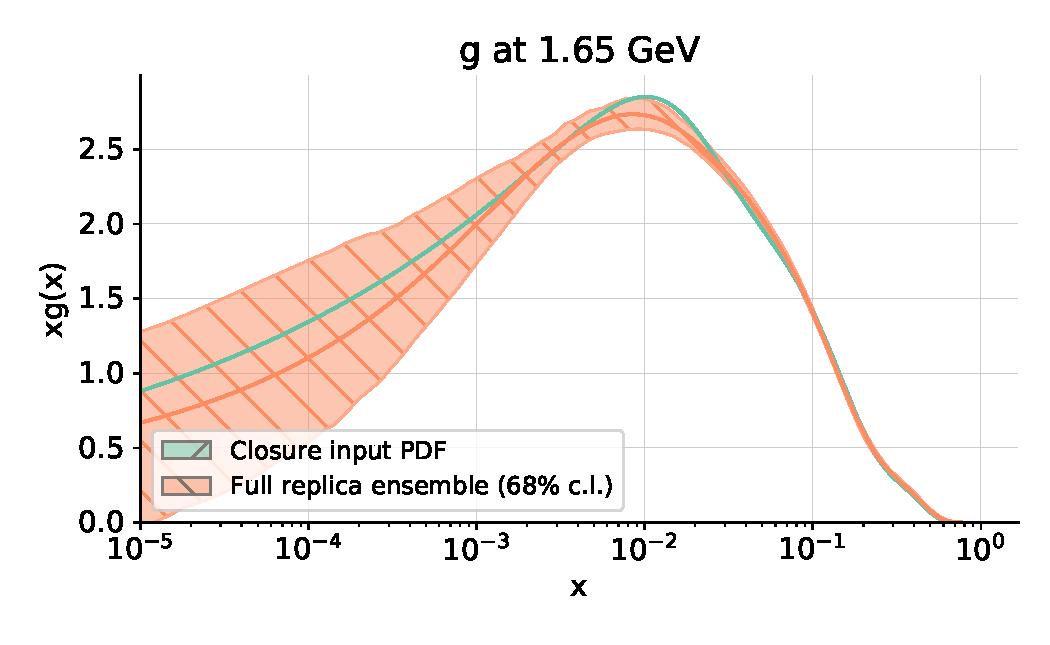
\includegraphics[scale=0.5]{closure_input_gluon.pdf}
    \caption{The green line is the input underlying law for the gluon PDF, which
    is sampled from the ensemble of replicas from a fit to data. The central
    value and the 68\% confidence interval for those replicas are plotted as the
    orange line and band respectively.}
    \label{fig:InputGluonPDF}
\end{figure}

The observables used in the fits are a subset of the full NNPDF4.0 dataset. For
convenience, we chose to fit the PDFs on a variant of the NNPDF3.1 dataset used
in Ref.~\cite{Ball_2018}, which is described in detail in a study of the
determination of the strange PDF~\cite{Faura_2020}. The datasets used in the
calculation of statistical estimators are the new datasets which have been
included in NNPDF4.0 and discussed in detail in the main release \cite{NNPDF40}. For a
full summary of the observables used in the test data and a visual representation of
the kinematic region of both the training and testing data, see
App.~\ref{sec:appendix-datasets}.

The partitioning of the available data into fitting and testing should not
affect the interpretation of the closure test results. However, one
could consider splitting the data into fitting and testing in a way which was
physically motivated \eg\ the partitioning could have been
stratified such that the kinematic coverage of the data of each partition
was approximately equal.
Alternatively, since the data is generated from the theory predictions produced
by the input underlying law, one could even produce completely artificial data
using a different set of FK tables. 

In order to compute the expectation value over training data defined in
Eq.~\ref{eq:average_over_training_data}, we generate 30 different sets of
experimental central values (or L1 data), as discussed in
Sec.~\ref{sec:closure-test-intro}, for the fitted 3.1-like dataset. Each set of
experimental central values was then fitted following NNPDF4.0 methodology
\cite{NNPDF40}, producing 40 pseudo-data replicas.


\subsection{Different components of the PDF uncertainty}

As already discussed in Ref.~\cite{nnpdf30}, fitting to L0, L1 and L2
pseudo-data allows us to validate different aspects of the fitting procedure. In
an L0 fit, we fit multiple time the exact same set of data, which corresponds to
the theory prediction from the chosen model. The fitted pseudo-data is the
result obtained by applying the forward map to the model. It is clear that in
this case the quality of the fit can be improved at will, provided that the
parametrization is flexible enough and the minimization algorithm is efficient.
There are indeed multiple solutions that reproduce exactly the data set, while
interpolating between the data points. In an L1 fit the data have been
fluctuated around the theoretical prediction -- mimicking thereby the central
values of experimental measurements. The true model no longer reproduces the
data; instead it will yield a $\chi^2$ of order one. The pseudo-data are held
fixed, fluctuations from one replica to the next are due to the existence of
multiple solutions that hold a similar value for the residual $\chi^2$ at the
end of the minimization process. Finally, in the L2 fits, the fluctuations of
the data are reproduced by the replicas, and propagated to the model function
when fitting the data for each replica. Since the NNPDF fitting methodology has
changed in the latest release, adopting the procedure described in
Ref.~\cite{Carrazza:2019mzf}, it is important to compare the uncertainties at
L0, L1 and L2 that are obtained with the NNPDF4.0 methodology with the
corresponding ones obtained with the NNPDF3.1 framework.

An example of these relative errors on fitted PDFs is shown in the upper panel of
Fig.~\ref{fig:CT_uncertainty_g} where results from L0, L1 and L2 closure tests
are displayed on the same plot in the case of the gluon distribution. Each fit
is normalized to the corresponding central value. We note how the L0 and L1
uncertainties tend to increase in the $x$ regions where less experimental data
are available, namely at small and large-$x$, where the model is left
unconstrained and has more freedom to fluctuate, while they are considerably
reduced in the data region where the contribution of the L2 error, induced by
the actual experimental data, becomes more important. The fact that the data
uncertainty is not always the dominant component of the PDF uncertainty was
already stressed in Ref.~\cite{nnpdf30}. Improved methodologies should therefore
aim to reduce the L0 and L1 error in the data region. Where 
less experimental data are available, we should still expect the dominant component 
of PDFs error to come from the L0 and L1 uncertainties, which however
should be driven by the lack of experimental information rather than by 
the unefficiency of the methodology.

In this respect, it is interesting to compare these results with what we find
with the NNPDF3.1 methodology. The corresponding plots are shown in the lower panel of
Fig.~\ref{fig:CT_uncertainty_g}: unlike the NNPDF4.0 case, here the PDF
uncertainty is always dominated by the L0 uncertainty, even in those kinematic
regions where experimental data are present. We can conclude that moving to the
NNPDF4.0 methodology, thanks to the optimized hyperparameters listed in Tab.~\ref{tab:Hyperparams},
we observe a marked reduction of the L0 uncertainty, 
see Fig.~\ref{fig:CT_uncertainty_new_vs_old}, where the latter is plotted on the same panel
for both NNPDF4.0 and NNPDF3.1. 
The better efficiency of the NNPDF4.0 methodology can be also appreciated
by looking at Fig.~\ref{fig:chi2_vs_epoch}, where we plot the distribution
across replicas of the L0 closure test $\chi^2$
as a function of the training epoch and genetic algorithm generation
for the NNPDF4.0 and NNPDF3.1 methodology respectively. As mentioned before, in a L0
closure test the quality of the fit can in principle be improved at will,
assuming the use of an efficient optimizer. For the final $\chi^2$ of the
central value of each fit, plotted as a black dashed line, we find $0.002$ and
$0.012$ in the NNPDF4.0 and NNPDF3.1 fitting code respectively, showing the better
efficiency of the new methodology. 

It should be noted how
Fig.~\ref{fig:CT_uncertainty_g}  only
provide a qualitative assessment of the relative size of the different
components of PDFs uncertainty. Despite being useful to assess how the
methodology has improved with respect to the previous one, they do not provide
any quantitative estimation of the faithfulness of PDF uncertainty. This is best
achieved in data space, using the new estimators introduced in the previous
sections.
How to validate PDFs uncertainty in the extrapolation regions remains an open problem,
and will be addressed in a future work.

\begin{figure*}[h]
    \centering
    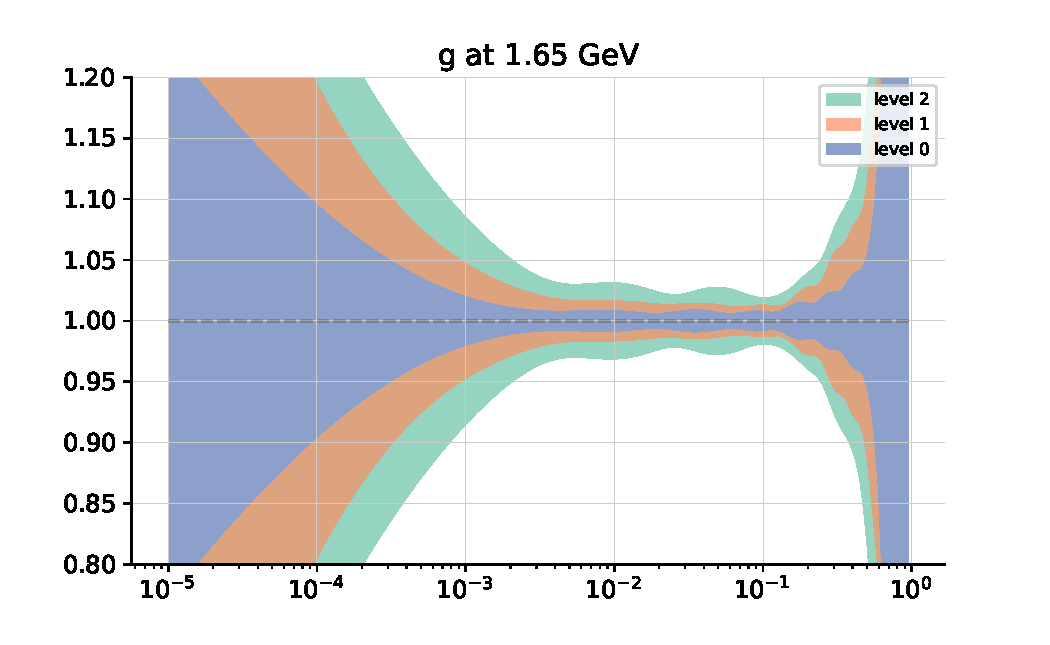
\includegraphics[scale=0.43]{CT_log_g.pdf}
    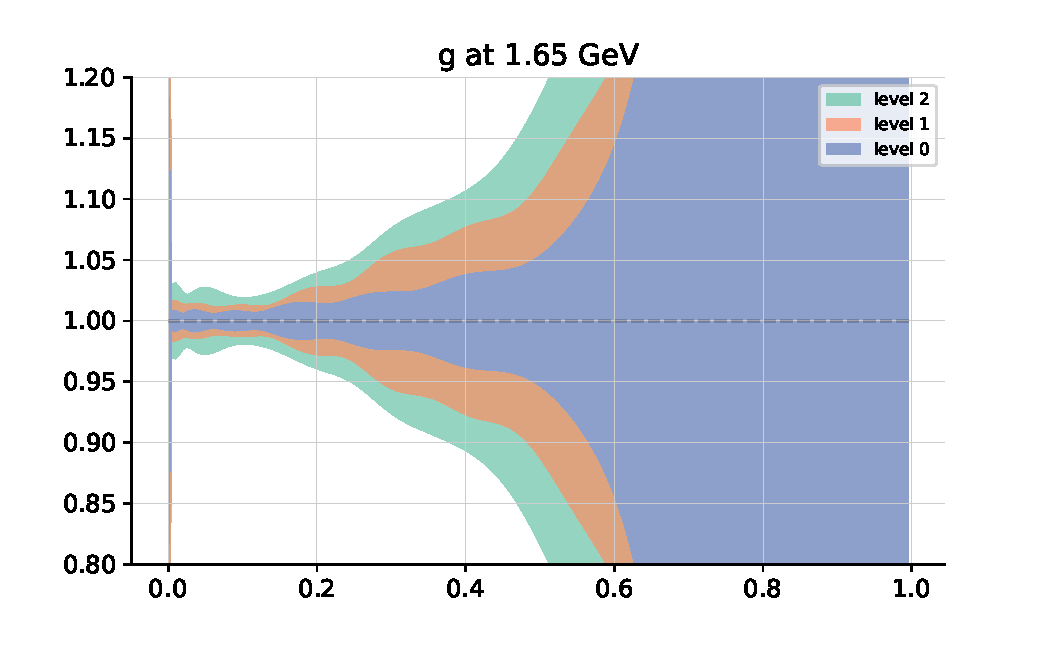
\includegraphics[scale=0.43]{CT_linear_g.pdf}
    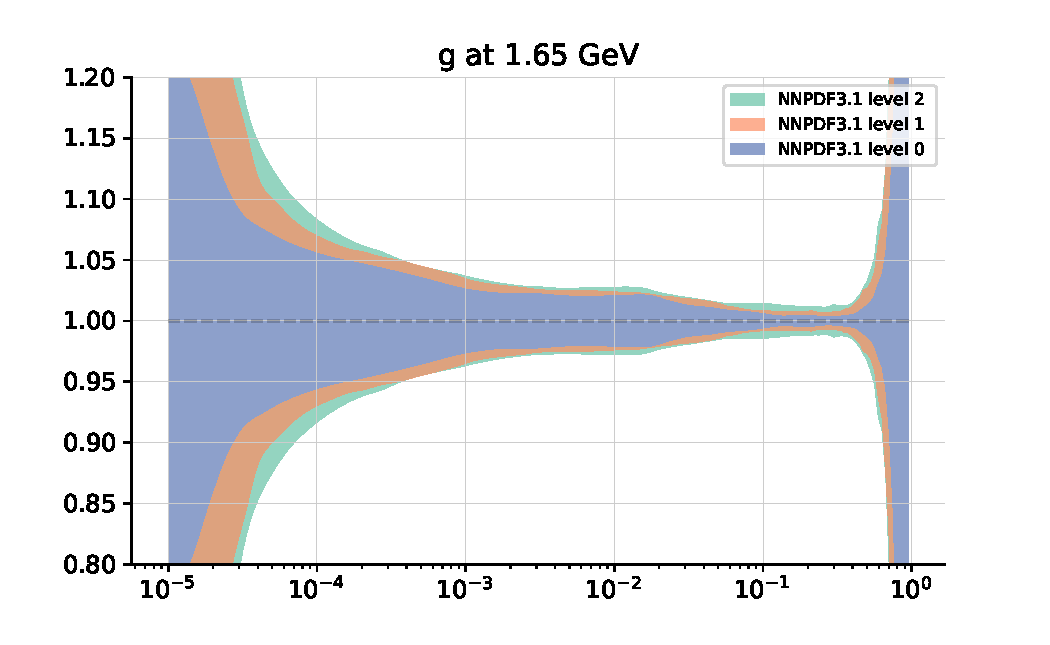
\includegraphics[scale=0.43]{CT_log_g_nnpdf31.pdf}
    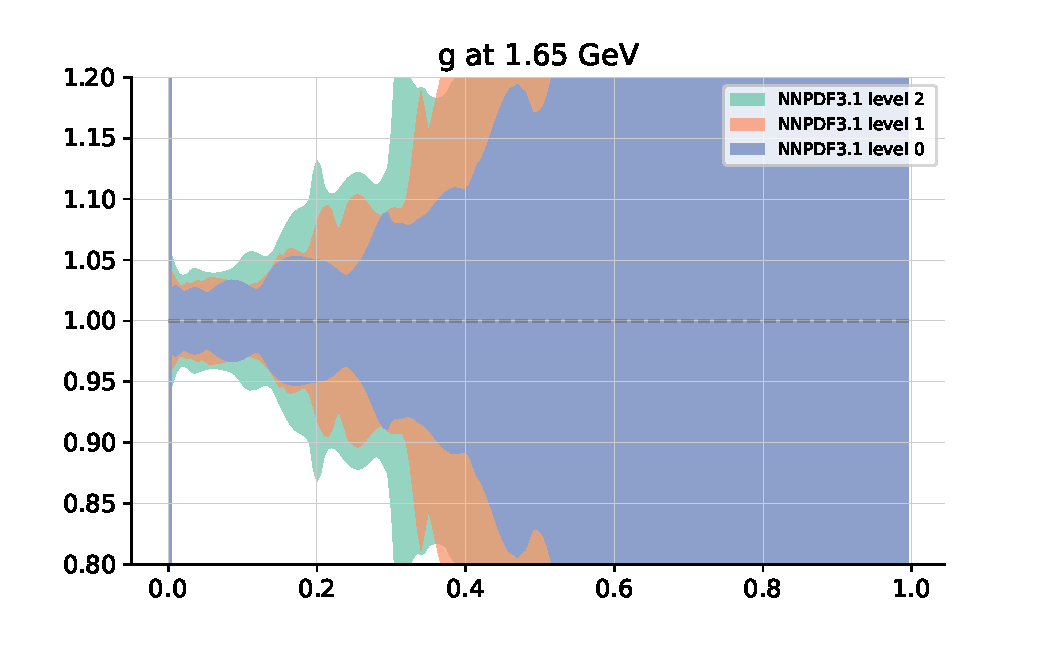
\includegraphics[scale=0.43]{CT_linear_g_nnpdf31.pdf}
    \caption{Relative PDF error for the gluon distribution in the NNPDF4.0 (upper panel)
    and NNPDF3.1 (lower panel) methodology, plotted in logarithmic (left) and linear scale (right).}
    \label{fig:CT_uncertainty_g}    
\end{figure*}

\begin{figure*}[h]
    \centering
    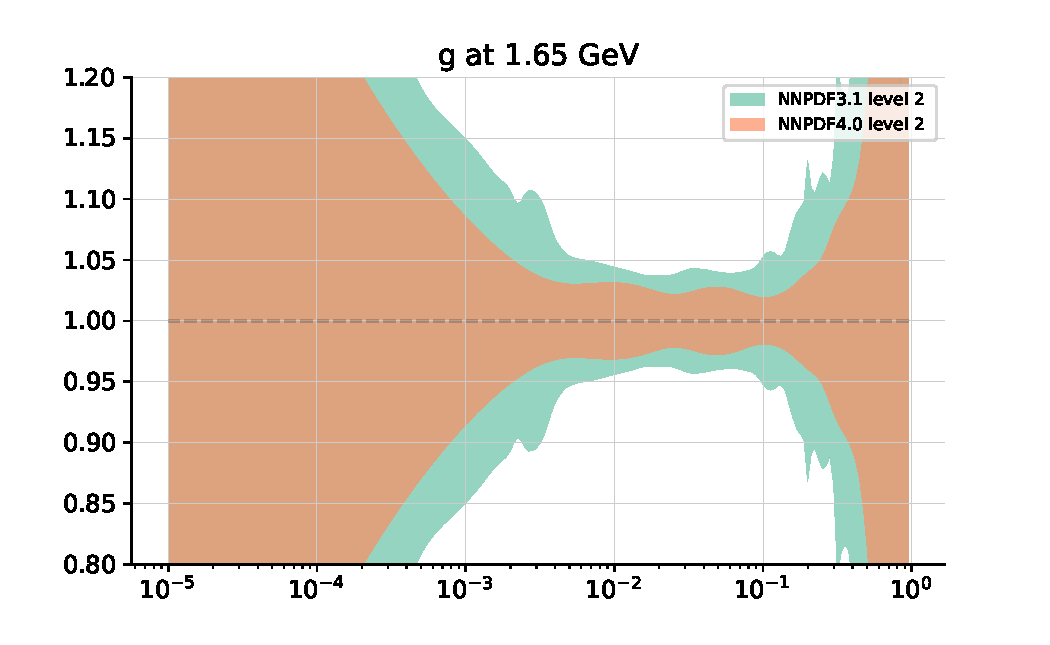
\includegraphics[scale=0.43]{CT_log_new_vs_old_g.pdf}
    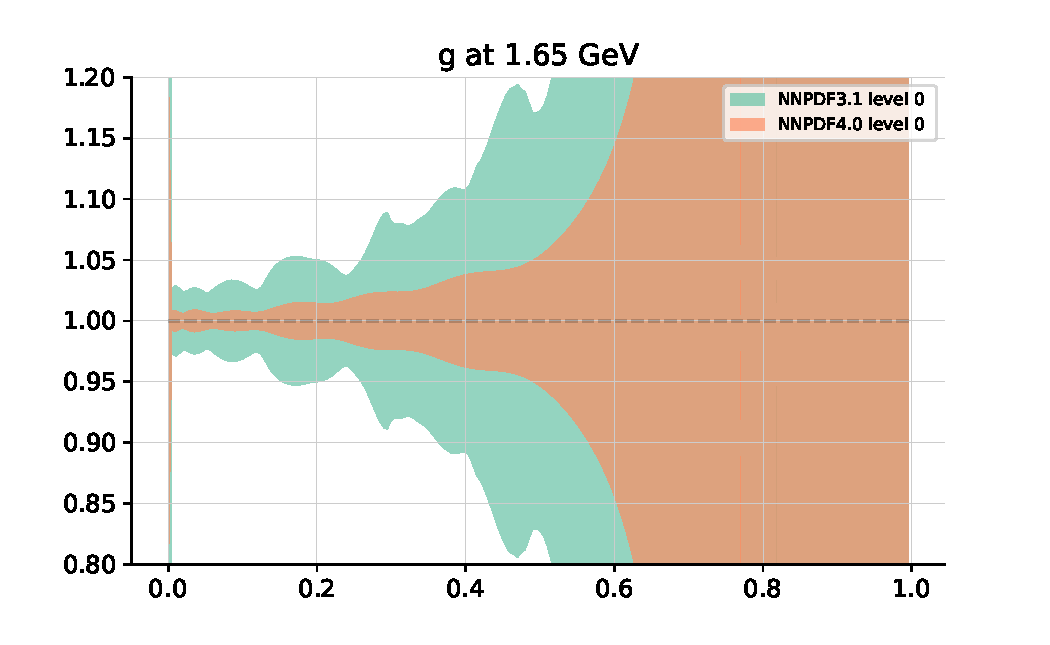
\includegraphics[scale=0.43]{CT_linear_new_vs_old_g.pdf}
    \caption{Level 0 uncertainty in the NNPDF4.0 and NNPDF3.1 methodology.}
    \label{fig:CT_uncertainty_new_vs_old}    
\end{figure*}

\begin{figure*}[h]
    \centering
    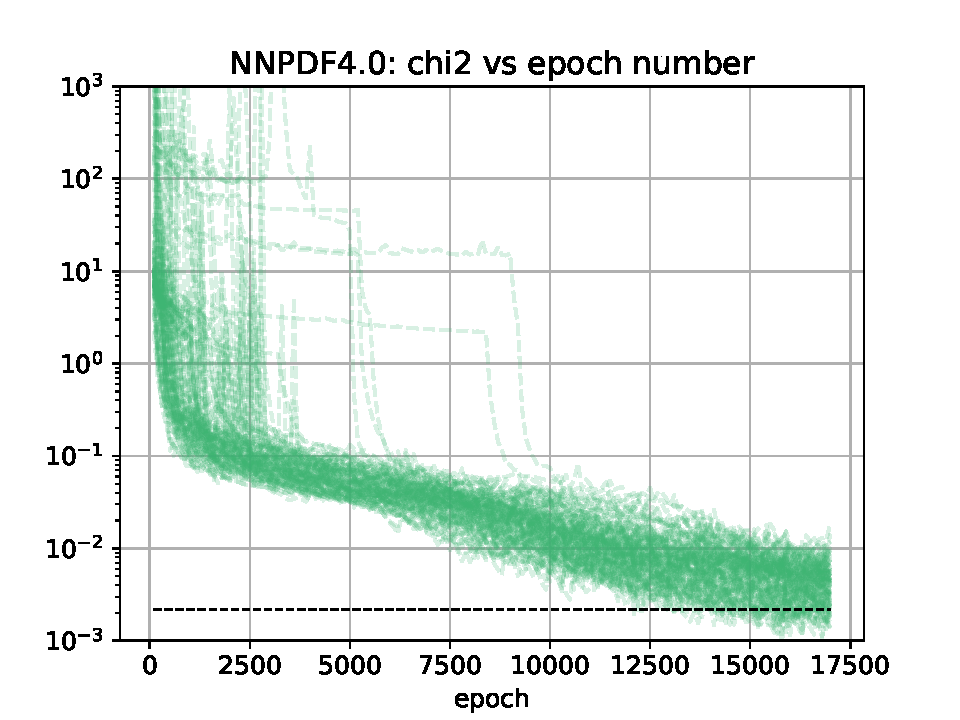
\includegraphics[scale=0.43]{chi2_n3fit_L0.pdf}
    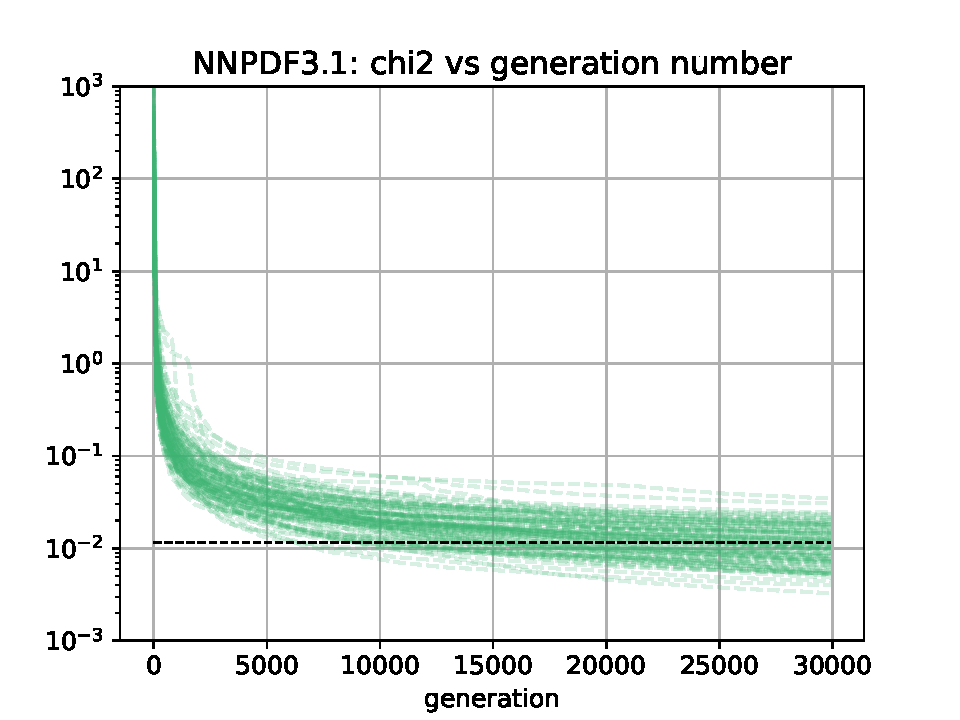
\includegraphics[scale=0.43]{chi2_nnfit_L0.pdf}
    \caption{$\chi^2$ distribution across replicas as a function of the training
    epoch and genetic algorithm generation for the NNPDF4.0 (left) and NNPDF3.1
    (right) methodology. The black dotted line
    in each plot represents the final $\chi^2$ of the central value of the
    corresponding fit, equal to $0.002$ and $0.012$ respectively.}
    \label{fig:chi2_vs_epoch}    
\end{figure*}



\subsection{Data space estimators}

Results for $\biasvarratio$ and the corresponding uncertainty calculated on the
test data are shown in the first column of Tab.~\ref{tab:biasvarratio}.
The uncertainties, which take into account the finite size of the replicas and fits samples,
have been computed by performing bootstrap, 
\cite{efron1994introduction}, where we randomly sample from both fits and
replicas and re-calculate $\biasvarratio$. The value and error presented in the
table is then the mean and standard deviation across bootstrap samples. We
checked that the distribution of the estimator across bootstrap samples is
indeed Gaussian. We also checked that increasing the number of fits and replicas
reduced the bootstrap error but the central values were the same within the
estimated bootstrap uncertainties. We see that overall $\biasvarratio$  is
consistent with 1, which gives a good indication that, at least for the unseen
data used in this study, the uncertainties are faithful

\begin{table}[h]
    \begin{center}
        \setlength{\tabcolsep}{12pt} 
        \begin{tabular}{rrr}
            \toprule
             $\biasvarratio$ & $\xi_{1\sigma}$ & $\erf(\biasvarratio/\sqrt{2})$ \\
            \midrule
             $1.03\pm0.05$ & $0.69\pm0.02$   & $0.67\pm0.03$                  \\
            \bottomrule
            \end{tabular}
    \end{center}
    \caption{In the first column we show the bias-variance ratio,
        $\biasvarratio$, for unseen data, summarised in
        Tab.~\ref{tab:summarise_new_data}. The uncertainty is estimated by
        performing a bootstrap sample across fits and replicas and calculating
        the standard deviation. We see that overall $\biasvarratio$ is
        consistent with 1, within uncertainties. In the second and third
        columns we compare the measured value of $\xi_1\sigma$ and the estimated
        value from $\biasvarratio$. The two values are consistent, which
        suggests the approximation that the ratio of uncertainties is
        approximately the same across all data is not completely invalidated.}
    \label{tab:biasvarratio}
\end{table}

In Fig.~\ref{eq:bias_varinace_distributions} we compare qualitatively the
distribution of bias across fits, to the distribution of the difference between
replica predictions and expectation values of predictions (in units of the
covariance) across different fits and replicas. The square root ratio of the
mean of these two distributions is precisely $\biasvarratio$.

\begin{figure}[h]
    \centering
    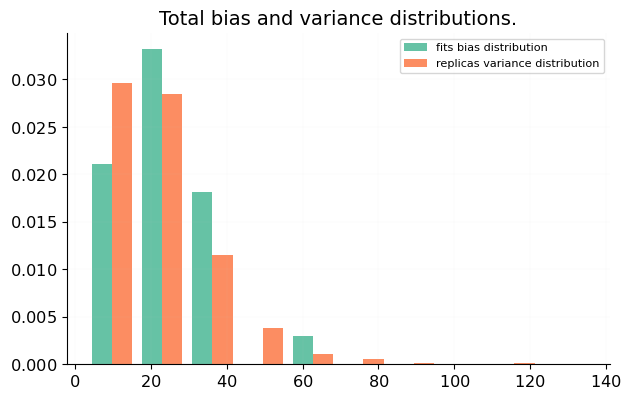
\includegraphics[scale=0.5]{plot_bias_variance_distributions_total.png}
    \caption{The green histogram is the distribution of the total bias across
    fits, the orange histogram is the distribution of the difference between the
    replica and central predictions squared, in units of the covariance across
    all fits and replicas. This gives a qualitative picture of the full
    distribution, in Tab.~\ref{tab:biasvarratio} we compare the square root of
    the mean of each distribution, getting the quoted value for
    $\biasvarratio$.}
    \label{eq:bias_varinace_distributions}
\end{figure}

As discussed in Sec.~\ref{sec:QuantileStatistics}, one can define an analogous
estimator in data space, based upon $\xi_{n\sigma}$, which was defined on a grid
of points in $x$ and $Q^2$ in PDF space in \cite{nnpdf30}. There is not a
one-to-one correspondence between this and $\biasvarratio$, but a loose
approximation using Eq.~\ref{eq:expectedxi}. In the second and third columns of
Tab.~\ref{tab:biasvarratio} we compare the estimated $\xi_{1\sigma}$ from
substituting $\biasvarratio$ into Eq.~\ref{eq:expectedxi} and to the measured
value. Despite the assumptions entering each of the two estimators differing, we
see good agreement between the $\xi_{1\sigma}$ estimated from $\biasvarratio$
and that measured directly. We find this result reassuring, since it indicates
not only that the total uncertainty averaged across all data is faithful, but
also that the uncertainty on each data point seems faithful. If the results
differed it would indicate some kind of imbalance, where some components of the
uncertainty are correctly represented by the replicas but other directions are
not. Finally we note how not only are the measured value and estimated value
from $\biasvarratio$ self consistent, but they are also consistent with $0.68$,
which further supports the argument that the model uncertainties are faithful.

%
As mentioned before, the improved efficiency of the new NNPDF4.0 code
makes it possible to easily compute the data space estimators for the new methodology,
but not for the NNPDF3.1 one, for which a much higher computational cost would be required to perform
the same exercise. For this reason, here we choose to present numbers for NNPDF4.0 only.
Given the fact that uncertainties in NNPDF4.0 are much smaller than those in NNPDF3.1,
one might still wonder to what extend such estimators can or cannot distinguish between
the two methodologies. In this respect, we notice that the faithfulness of uncertainties as defined here
is not directly related to the corresponding size, and that the estimators presented here
cannot distinguish between two different faithful methodologies. 
Looking at the toy example of Fig.~\ref{fig:diagram2destimators}, if we had bigger uncertainty, like 
in the NNPDF3.1 case, we would expect to get a bigger blue circle, with the true value of the observable
still within its larger $68\%$. The data space estimators for any faithful methodology
should therefore have similar values to those obtained for NNPDF4.0, independently of the
relative size of the uncertainty.





